\cotefile{136}
\scanpage{330}

\diagram{\begin{tikzcd}
\Gamma^p(\Gamma^q(X)) \\
\Gamma^{pq}(X)\arrow[u,"{\deleted{\beta}\inserted{\gamma}^{X}_{p,q}}"']
\end{tikzcd}}

\diagram{\begin{tikzcd}
\beta^X_{p,q}:\ \Gamma^p(X)\otimes\Gamma^q(X)\arrow[r] & \Gamma^{pq}(X) \\
\alpha^{X,Y}_{pq}:\ \Gamma^{\unsure{*|p}}(X)\otimes\Gamma^*(Y)\arrow[r,"\sim"] & \Gamma^{2}(X\times Y)
\end{tikzcd}}

\[\Delta:\ A\longleftarrow A\otimes A\]
\[u_p:\ A\longleftarrow\Gamma^p A\]
\diagram{\begin{tikzcd}
F(X\otimes Y) & F(X)\otimes F(Y)\arrow[l,"\tau_{X,Y}"'] \\
F(\Gamma^p(X)) & \Gamma^pF(X)\arrow[l,"\sigma^{\alpha}_p"']
\end{tikzcd}}
OK\quad OK

\par\noindent\rule{.9\linewidth}{.3pt}

\deleted{Soit $A$ algèbre sur un anneau $k$ \deleted{de car. $0$}, on va définir un hom can. \deleted{$k$-lin.}
\[
\operatorname{Sym}^*A\longrightarrow A
\]
par ses restrictions
\[
\operatorname{Sym}^n(A)\xrightarrow{u_n} A\qquad(n\geq0)
\]
et en prenant
\[
u_n(\underbrace{x_1.x_2.\ldots.x_n}_{\substack{\text{produit}\\\text{dans }\operatorname{Sym}^*(A)}})
=\frac1{n!}x_1x_2\ldots x_n
\]
Je dis que le diagramme
\diagram{\begin{tikzcd}[column sep=large,row sep=large]
\operatorname{Sym}^{p+q}A\arrow[r,"C_{pq}u_{p+q}"]\arrow[d,"\Delta"'] & A \\
\operatorname{Sym}^pA\otimes\operatorname{Sym}^qA\arrow[r,"u_p\otimes u_q"'] & A\otimes A\arrow[u,"\text{mult. de }A"']
\end{tikzcd}}

i.e un hom can. de
\[
\deleted{(\Gamma^\alpha(A)\otimes A)^{\wedge}}
\]
\[
\deleted{\Gamma^\alpha,\,V(A)}\operatorname{Hom}_{k\text{-lin}}(\operatorname{Sym}^*A,B
\]
\[
=\Gamma^*(\check A)\otimes_k B\qquad\text{i.e.}\ \text{un élt}\ \text{de}
\]
\[
\Gamma^*(\check A)\otimes B\qquad\text{p. ex.}\text{ de }\check A\otimes_k B
\]
\deleted{\unsure{$u$}}
\[
A\underset{\unsure{h|k}}{\Longrightarrow} B\qquad k\text{ lin.}
\]
\[
\operatorname{Sym}^* A
\]
\[
\operatorname{Sym}^*(
\]
}

\mspage{331}
\scanpage{332}

\diagram{\begin{tikzcd}
\Gamma^*F(X)\arrow[r,"u_*"] & F\Gamma^*X \\
\Gamma^pF(X)\arrow[r,"u_p",no head] & F\Gamma^p(X)
\end{tikzcd}}

\deleted{$x^{(p)}$}
\diagram{\begin{tikzcd}
F(X)\arrow[r,"!"] & F\Gamma^p(X)
\end{tikzcd}}
\[x\in F(X)\qquad\deleted{1}\qquad\text{degré }p\]
\[
u_p(\gamma^p_{F(X)}(x))=F(\gamma^p_X)(x)
\]
\diagram{\begin{tikzcd}
X\arrow[r] & \Gamma^p(X)
\end{tikzcd}}
\[\text{degré }p\]
\[
u_*(\gamma^p_{F(X)}(x))=F(\gamma^p_X)
\]

\deleted{$u_p\ \&$}
\diagram{\begin{tikzcd}[column sep=huge,row sep=large]
\Gamma^pF(X)\arrow[r,"u_p"]\arrow[d,"{\xi\mapsto\xi^{(q)}}"]\arrow[dd,bend right=45,no head,"{\xi\mapsto\gamma^q(\xi)}"'] & F(\Gamma^p(X))\arrow[d,"{F(\eta\mapsto\eta^{(q)})}"] \\
\Gamma^{pq}(F(X)).\arrow[r,"u_{pq}",no head] & F(\Gamma^{pq}(X)) \\
\Gamma^q(\Gamma^pF(X)) &
\end{tikzcd}}

\[
u_p(\gamma^p(x))=F(\gamma_X^p)(x)
\]
\[
F(\gamma_X^{q,p})(F(\gamma_X^p)(x)
\]
\[
F(\gamma_X^{q,p}\gamma_X^p)(x)\ \}
\]
\[\text{''}\]
\[
F(\alpha_{pq}\gamma_X^{pq})(x)=\alpha_{pq}F(\gamma_X^{pq})(x))
\]
\margin{$\begin{gathered}\Vert\\\displaystyle\frac{(pq)!}{(p!)^q q!}\end{gathered}$}
\[
\begin{aligned}
&=\!=\!.\ \alpha_{pq}\,\deleted{u}\,u_{pq}(\gamma^{pq}(x))\\
&=u_{pq}(\alpha_{pq}\gamma^{pq}x)\\
&=u_{pq}(\gamma^{q,p}_{F(X)}(\gamma^p_{F(X)}(x))
\end{aligned}
\]

de $=$ pr
\[
\uline{u_*(\gamma^{\alpha_1}(x_1)\ldots\gamma^{\alpha_n}(x_n))}
\]

\[\text{''}\]
\[
u(\lambda)^{pq}\,u(\alpha_{pq}x^{(pq)})
\]
\margin{$\text{''}\quad u(\lambda)^{q}\alpha_{pq}\,u(x)^{pq}$}
\[
\lambda^{pq}\alpha_{pq}\,u(x_{i}^{\deleted{(pq)}})^{(pq)}
\]

\mspage{333}
\scanpage{333}

\[
u_{\deleted{pq}\inserted{*}}\bigl((\sum\xi_i)^{(q)}\bigr)
\overset{?}{=}(\sum u_*(\xi_i))^{(q)}
\]
\[\text{''}\qquad\text{''}\]
\[
u_{pq}\bigl(\sum\xi_1^{(q_1)}-\xi_r^{(q_r)}\bigr)
=\sum u_{\unsure{*|q_1}}(\xi_1)^{(q_1)}-u_*(\xi_r)^{(q_r)}
\]

On est ramené à prouver que
\[
u_*(\xi_i^{(q_i)})=u_*(\xi_i)^{(q_i)}
\]
pour les \unsure{sommants|sommands}, ts $q^i$.
Cela revient au cas
\[
\xi_i=x_1^{(p_1)}-x_r^{(p_r)}
\]
\[
u_*\bigl(\underbrace{(x_1^{(p_1)}-x_r^{(p_r)})^{(q)}}_{\substack{\Vert\\(x_1^{(p_1)}-x_{r-1}^{(p_{r-1})})^q(x_r^{p_r})^q}}\deleted{\longrightarrow}\bigr)
\overset{?}{=}u_*(x_1^{(p_1)}-x_r^{(p_r)})^{(q)}
\]

\[
u_*\bigl(\underbrace{(x_{p}^{(p)})^{(q)}}_{\alpha_{pq}x^{(pq)}}\bigr)\ =\ u
\]
\margin{$\deleted{u(\alpha_{pq}x^{(pq)})=}\quad\Vert$}
\[
u\bigl((x^{(p)})^{\deleted{(q)}}\bigr)
=u(x\deleted{q}^{(p)}\deleted{^{(q)}})
\]
\[\Vert\]
\[
F(\gamma_{\unsure{a|\alpha}}^p)(x)=x^{(p)}
\]

\diagram{\begin{tikzcd}[row sep=small]
A\arrow[r,"u"] & B \\
\deleted{u}J\arrow[u,phantom,"\cup" description]\arrow[r] & K\arrow[u,phantom,"\cup" description]
\end{tikzcd}}
\margin{$u$ compatible aux pd.\qquad $u(x$}
\[(x_i)_{i\in I}\]

$J$ engendré par les $x_i$ comme idéal à pd.
i.e. comme idéal engendré par les
\[
x_i^{(p)}\qquad(p\geq1)
\]
\[
\unsure{\Downarrow|Si}\qquad u(x_i^{(p)})=u(x_i)^{(p)}\qquad\mathrm{OK}
\]
\[
u\bigl((\sum\underbrace{\lambda_i x_i^{(p_i)}}_{\xi_i})^{(q)}\bigr)
\overset{?}{=}\bigl(u(\underbrace{\sum\lambda_i x_i^{(p_i)}}_{\xi})\bigr)^{(q)}
\]
\[
u\bigl(\sum\xi_1^{(q_1)}-\xi_r^{(q_r)}\bigr)
=\sum u(\xi_1)^{(q_1)}-u(\xi_r)^{(q_r)}
\]
Il suffit
\[
u(\xi_i^{(q_i)})=u(\xi_i)^{(q_i)}
\]
OPS.\quad $x=\lambda_i x_i^{(p)}$
\[
u(x^{(q)})=u(x)^{(q)}
\]
\[
u\bigl(\lambda^q(x_i^{(p)})^{(q)}\bigr)
=u(\lambda)^q\bigl(u(x_i)^{(p)}\bigr)^{(q)}
\]

\mspage{334}
\scanpage{334}

Plus gén., si $A\supset J$ est un anneau à pd., on a $F(J)\longrightarrow F(A)$ inj., donc $F(J)$ à p. div. dans $F(A)$ ?

\diagram{\begin{tikzcd}
F(J)\arrow[r,"\mathrm{deg}\ p"] & F(J) \\
J\arrow[r,"\gamma^p",no head] & J
\end{tikzcd}}
\margin{oui, en \unsure{transf.|transportant}}

\deleted{\unsure{F}}\unsure{Je trouve la relation|Je donne la relation}
\deleted{$(x+y)$}
\[
x,y\in F(J)\quad\Longrightarrow\quad
(x+y)^{(p)}\overset{!}{=}\sum_{i+j=p}x^{(i)}y^{(j)}\quad?
\]
\[x,y\in\qquad\Vert\qquad u\]

\diagram{\begin{tikzcd}
\mathcal P\arrow[r,"\overline F",no head] & \mathcal P'
\end{tikzcd}}
commute aux produits\par
conserve degré et degrés partiels
\margin{bidegrés $1,1$}

\deleted{donc il}
\[
A,J\qquad J\longrightarrow A
\]
$A$ \deleted{ab. groupe} \inserted{$k$-} ass comm avec $1$\par
$J$ anneau ass comm sans $1$\par
$A$ opère sur $J$, et $(\lambda xy=x(\lambda y)=\lambda xy$
\[
J\xrightarrow{i} A\qquad\text{hom de }A\text{-}\text{algèbre}
\]
\[
(i(xy)=i(x)i(y)\qquad i(\lambda x)=\lambda i(x))
\]
\margin{\diagram{\begin{tikzcd}
A\times A\arrow[r] & A \\
A\times J\arrow[r] & J
\end{tikzcd}}}
\[
k\longrightarrow\operatorname{Hom}_{\mathcal P}(0,A)\qquad\text{hom d'anneaux}
\]
\deleted{\unsure{propre}}
\[
\gamma^p:\ J\xrightarrow[\text{degré }p]{}J\qquad p\geq1
\]
\margin{$\gamma^0:J-A$}
\[
\begin{aligned}
\gamma^0&=1\\
\gamma^1&=\mathrm{id}_J\\
\gamma^p(x+y)&=\sum_{i+j=p}\gamma^i x\,\gamma^j y\\
\gamma^p(\lambda x)&=\lambda^p\gamma^p(x)\\
\gamma^p(x)\gamma^q(x)&=C_{pq}\gamma^{p+q}(x)\\
\gamma^p(\gamma^q(x))&=\frac{(pq)!}{(p!)^q q!}\gamma^{pq}(x)
\end{aligned}
\]

\uline{transformé en Ann}
\diagram{\begin{tikzcd}
\Gamma^*F(X)\arrow[r] & F\Gamma^*(X)
\end{tikzcd}}

\mspage{335}
\scanpage{335}

\diagram{\begin{tikzcd}
\Gamma^p F(X) \arrow[r,"u_p^X"] & F(\Gamma^p(X))
\end{tikzcd}}
\[
x\in F(X)\longmapsto x^{(p)}=u_p^X(\gamma^p(x)).
\]
\[
u_*^X:\quad \Gamma^*F(X)-
\underbrace{F(\Gamma^*(X))}_{\substack{\text{Algèbre car}\\
\text{F compatible à }\otimes\ \text{donc transforme}\\
\text{alg. en alg.}}}
\qquad \text{hom d'algèbres}
\]

cela \deleted{signifie} \inserted{implique} que
\[
(x+y)^{(p)}=\sum_{i+j=p}x^{(i)}\otimes y^{(j)}.
\]
\diagram{\begin{tikzcd}
F(P)\otimes F(Q) \arrow[d] & \\
F(P\otimes Q) \arrow[r,no head] & F(R)
\end{tikzcd}}
\[
\begin{aligned}
&\text{''}\\
u_*\bigl(\underbrace{\gamma_p(x+y)}_{\sum_i\gamma_i(x)\gamma_j(y)}\bigr)
&=\sum_i u_*\bigl(\gamma_i(x)\gamma_j(y)\bigr)\\
&=\sum\underbrace{u(\gamma_i(x))}_{x^{(i)}}\,
\underbrace{u(\gamma_j(y))}_{y^{(j)}}
\end{aligned}
\]
\[
(\lambda x)^{(p)}=\lambda^p x^p
\]
\[
\begin{gathered}
\text{''}\\
u_p^X\gamma^p(\lambda x)=u_p^X(\lambda^p\gamma^p(x))
=\lambda^p u_p^X(\gamma^p(x))=\lambda^p x^{(p)}
\end{gathered}
\]
\[
x^{(p)}x^{(q)}=c_{pq}x^{(p+q)}\quad ?
\]
\[
\begin{aligned}
&\text{''}\\
u_*\gamma^p(x)\,u_*\gamma^q(x)
&=u_*\bigl(\underbrace{\gamma^p(x)\gamma^q(x)}_{c_{pq}\gamma^{p+q}(x)}\bigr)
=c_{pq}u\gamma^{p+q}(x)\\
&=c_{pq}x^{(p+q)}
\end{aligned}
\]

\figure{\begin{tikzpicture}
\draw (0,0) .. controls (2,-.04) and (4,.14) .. (5,.12)
.. controls (5.8,.18) and (5.3,-.65) .. (6.4,-.65)
.. controls (8,-.72) and (9,-.65) .. (10,-.68);
\draw (.2,0) -- (.2,-.35) -- (.15,-.45) -- (.2,-.65);
\end{tikzpicture}}
\[
\uline{1}-F(\uline{1})
\]
\diagram{\begin{tikzcd}
\Gamma^*F(X) \arrow[r] & F\Gamma^*(X)\\[-1ex]
F(X) \arrow[r,"\mathrm{id}"] & F(X)
\end{tikzcd}}
mult., \unsure{bien} gradué

\unsure{respecte-t-il} les p.d. ?

\margin{$F\Gamma^*(X)$ a-t-il un p.d.}

\diagram{\begin{tikzcd}[row sep=large,column sep=huge]
\Gamma^pF(X) \arrow[r,"u_p^{F(X)}"]
\arrow[d,"\gamma^q_{\Gamma^pF(X)}"'] & F\Gamma^p(X)
\arrow[d,"F(\gamma^q_{\Gamma^p(X)}" ]\\
\Gamma^q\Gamma^pF(X) \arrow[d] & F(\Gamma^q(\Gamma^p(X)))\\
\Gamma^{qp}F(X) &
\end{tikzcd}}
\figure{\begin{tikzpicture}\draw (0,.9) .. controls (.5,.9) and (.7,.55) .. (1,0);\end{tikzpicture}}

\mspage{336}
\scanpage{337}

\diagram{\begin{tikzcd}[column sep=large,row sep=large]
& \Lambda^n\Psi_* \arrow[r] & \Lambda^{n+1}\Phi_*=C_*^n\\
\Lambda^{n-1}\Psi_* \arrow[r,"T_\Lambda","\text{mono}"'] &
\Phi_*\otimes\Lambda^{n-1}\Psi_* \arrow[u] \arrow[r] & \Lambda^n\Phi_*=C_*^{n-1}\arrow[u]\\
\Phi'_*\otimes\Lambda^{n-2}\Psi_* \arrow[u] \arrow[r] &
\Gamma^2\Phi_*\otimes\Lambda^{n-2}\Psi_* \arrow[u] \arrow[r] &
\Lambda^{n-1}\Phi_*=C_*^{n-2}\arrow[u]
\end{tikzcd}}
\[
(\Lambda^n\Phi_*)^n\ \unsure{\simeq}
\]
\[
(\Lambda^n\Phi_*+\unsure{S|\S}(\Lambda^{n-1}\Phi_*)^{\frac{n(n-1)}2}
\]

\[
(N+1)\binom{N}{n-1}
=\frac{(N+1)N---(N-n+2)}{(n-1)!}
=n\binom{N+1}{n}
\]
\[
\frac{(N+1)(N+2)}2\binom{N}{n-2}
=\frac{\overbrace{(N+2)(N+1)N-\deleted{N}(N-n+3)}^{n\ \text{fact.}}}
{\deleted{(n-2)!}\inserted{n!}}\ \frac{n(n-1)}2
=\binom{N+2}{n}\frac{n(n-1)}2
\]

\[
\operatorname{rg}\bigl(\Gamma^p\Phi_{[N]}\otimes\Lambda^q\unsure{\Psi_{[N]}\prime|\Psi_{[N]})}
=\frac{(N+1)(N+2)--(N+p)}{p!}
\frac{N\deleted{\unsure{+}}(N-1)-(N-q+1)}{q!}
\]
\[
\unsure{\simeq}
\]
\[
\deleted{\unsure{(1+t)^N=1+nt+\frac{n(n-1)}2}}
=\frac{(N+p)---(N-q+1)}{(p+q)!}\frac{(p+q)!}{p!q!}
=c_{pq}\binom{N+p}{p+q}-
\]

\[
(\tau P)(\mu)=P(\mu+1)
\]
\margin{\deleted{\unsure{Ainsi}}
\[
\begin{aligned}
\varphi_{p+q}(N+p)&=\varphi_{p+q}(N+p-1)+\varphi_{p+q-1}(N+p-1)\\
&=\varphi_{p+q}(N+p-2)+2\varphi
\end{aligned}
\]}
\[
\tau\varphi_r=\varphi_r+\varphi_{r-1}
\]
\[
\begin{aligned}
\tau^2\varphi_r&=\tau\varphi_r+\tau\varphi_{r-1}
=\begin{gathered}\varphi_r+\varphi_{r-1}\\+\varphi_{r-1}+\varphi_{r-2}\end{gathered}
=\varphi_r+2\varphi_{r-1}+\varphi_{r-2}
\end{aligned}
\]
\[
\begin{aligned}
\tau^3\varphi_r&=\varphi_r+\varphi_{r-1}\\
&\qquad+2\varphi_{r-1}+2\varphi_{r-2}\\
&\qquad\qquad+\varphi_{r-2}+\varphi_{r-3}\\
&=\varphi_r+3\varphi_{r-1}+3\varphi_{r-2}+\varphi_{r-3}-
\end{aligned}
\]

\margin{\[
=c_{pq}\underbrace{\tau^{p-1}_{\deleted{\unsure{*}}}\varphi_{p+q}}(N+1)
\]
\[
\deleted{=\unsure{c_{pq}\tau}}\qquad
\deleted{\unsure{\tau^{p-1}}}
\]}
\figure{\begin{tikzpicture}
\draw (0,4) -- (.65,1.3);
\draw (.65,.3) -- (.52,-.1);
\node at (.52,-.35) {$2$};
\draw (.47,-.6) -- (.22,-1.45);
\end{tikzpicture}}

\[
\tau^p\varphi_r=\varphi_r+p\varphi_{r-1}
+\deleted{\unsure{\frac{p(p-1)}2}}\inserted{\binom p2}\varphi_{r-2}
-+\varphi_{r-p}
\]
\[
\tau^{p-1}\varphi_{p+q}=\varphi_{p+q}+(p-1)\varphi_{p+q-1}-+\varphi_{q+1}
\]
\[
c_{p,q}\bigl(\Lambda^{p+q}\Phi_*+(p-1)\Lambda^{p+q-1}\Phi_*
+\binom{p-1}{2}\Lambda^{p+q-2}\Phi_*-+\Lambda^{q+1}\Phi_*\bigr)
\]

\mspage{338}
\scanpage{338}

\margin{$\operatorname{Hom}^!(\Delta^m,\Delta^n)=$ ens des applications croissantes
$\Delta^m\longrightarrow\Delta^n\deleted{=}[0,n]$
l'image est égale à $\Delta^n$ (i.e surj) ou à $[0,n-1]$}

\diagram{\begin{tikzcd}[column sep=large,row sep=large]
& \mathbb C_*^* \arrow[dl] &\\
\mathbb C_\bullet^* && C_*^\bullet=\Lambda^{\bullet+1}\Phi_* \arrow[ul,hook]\\
& C_\bullet^\bullet \arrow[ul,hook] \arrow[ur,hook] &
\end{tikzcd}}
\[
\left\{\begin{aligned}
\mathbb C_{[n]}^*&=\mathbb C^*(\Delta_*^n)=k_*(\Delta_*^n)=k_*^{\Delta_*^n}\\
\mathbb C_*^{(m)}&=p_{m*}(k)=(n\longmapsto k^{\operatorname{Hom}_\Delta(\Delta^m,\Delta^n)}
\end{aligned}\right.
\]
\[
\left\{\begin{aligned}
C_{[n]}^\bullet&=C^\bullet(\Delta^n)=\Lambda^{\bullet+1}k^{\Delta^n}\\
C_*^m&=\Lambda^{1+m}\Phi_*
\end{aligned}\right.
\]
\[
\left\{\begin{aligned}
C_\bullet^m&\simeq k\ \text{en degrés }m,m+1)\\
C_{\unsure{m|n}}^\bullet&\simeq
\begin{cases}k\ \text{en degrés }n,n-1\quad(n\geq1)\\
k\ \text{en degré }0\quad\text{si }n=0
\end{cases}
\end{aligned}\right.
\]
(dans $(K_\bullet)^\bullet$; complexes de \uuline{colonnes})
\[
C_\bullet^\bullet
\]

\diagram{\begin{tikzcd}[column sep=huge,row sep=huge]
& \mathbb C_{[n]}^{(m)}=k^{\operatorname{Hom}_\Delta(\Delta^m,\Delta^n)} \arrow[dl] &\\
\mathbb C_n^{[m]}=k^{\inserted{\operatorname{Hom}^!}\deleted{\unsure{\operatorname{Hom}}}(\Delta^m,\Delta^n)}
&& C_{[n]}^m=\Lambda^{m+1}k^{\Delta^n}
=k^{\operatorname{Inj}_\Delta(\Delta^m,\Delta^n)}
\arrow[ul,hook,"\text{iso \uline{seulement} si }m=0"']\\
& C_n^m \arrow[ul,hook,"\text{iso si }n\geq m+1"]
\arrow[ur,hook,"\text{iso si }m\geq n"'] &
\end{tikzcd}}
\margin{fact. dir. can.}
\deleted{\text{et iso can.}}
\[
\begin{gathered}
\text{nul si }n>m+1\\
\simeq k\ \text{si }n=m+1
\end{gathered}
\qquad
(\text{nul si }m>n,\ =k\ \text{si }m=n)
\]
\[
C_n^m=
\begin{cases}
0\ \text{si }n\ne m,m+1\\
k\ \text{si }n\begin{cases}=m\\=m+1\end{cases}
\end{cases}
\]
alors
\[
C_{[m]}^m=\Lambda^{m+1}k^{m+1}\simeq k
\]
alors
\[
C_{m+1}^m=\Lambda^{m+1}k^{m+2}\simeq k^{m+2}
\]
et \unsure{on a} l'injection diagonale sans doute

\figure{\begin{tikzpicture}
\draw (.2,1.6) .. controls (-.15,.8) and (-.15,.5) .. (.55,0);
\draw (0,-.4) .. controls (-.3,-1.1) and (2,-.9) .. (2.8,-1.2);
\end{tikzpicture}}

\[
\operatorname{Hom}_*(X_*,\underset{\cup}{\mathbb C_*^{[i]}})
\simeq\mathbb C^{[i]}(X_*)\simeq k^{X_{[i]}}
=\operatorname{Hom}_{\mathrm{ens}}(X_{[i]},k)
\]
\[
\operatorname{Hom}_*(X_*,C_*^i)\simeq\operatorname{Hom}(X_*,\Lambda^{i+1}\Phi_*)
\overset{\supset}{=}\underbrace{C_a^i(X_*)}_{\text{sous-entendu}\ C_*^i}
\]
\[
\mathbb C_*(X_*)\overset{\mathrm{d\acute ef}}{=}k(X_*)=k^{(X_*)}
=(n\longmapsto k(X_{[n]})=k^{(X_{[n]})})
\]
donc
\[
\mathbb C^*(X_*)\simeq\mathbb C_*(X_*)^\vee
=(n\longmapsto(k^{(X_{[n]})})^\vee=k^{X_{[n]}})
\]
\[
C_\bullet(X_*)\subset\mathbb C_a(X_{\bullet}),\quad
\text{on a}\quad C^\bullet(X_*)\simeq C_\bullet(X_*)^\vee
\]
\diagram{\begin{tikzcd}
C_\bullet(X_*) \arrow[dr,equal,"\text{fact. dir. can.}"] &\\
&\operatorname{ND}(\mathbb C_*(X_*))
\end{tikzcd}}

\diagram{\begin{tikzcd}[column sep=large,row sep=large]
& \mathbb C_*^*=\mathbb C_*^{*\vee}\arrow[dl] &\\
\mathbb C_*^\bullet=\mathbb C_\bullet^{*\vee} &&
C_\bullet^*=C_*^{\bullet\vee}=(\Lambda^{\bullet+1}\Phi_*)^\vee
\arrow[ul,hook] \arrow[dl]\\
&\mathbb C_\bullet^\bullet=C_\bullet^{\bullet\vee}\arrow[ul,hook]&
\end{tikzcd}}
\[
(C_m^\bullet=k\ \text{en deg }m,m\unsure{+|-}1)
\]
(dans $(K_\bullet)^\bullet$; $C_\bullet^\bullet$ est complexe de \uuline{chaînes} \unsure{unité|mixte})
\[
C_\bullet^n=\begin{cases}
k\ \text{en degrés }n,n-1\quad(n\geq1)\\
k\ \text{en degré }0\quad(n=0)
\end{cases}
\qquad\deleted{\unsure{k}}
\]

\mspage{339}
\scanpage{339}

À tout $X_*\in\operatorname{Ob}\widehat\Delta=\operatorname{Ob}S_s$,
on associe le foncteur
\[
F_{X_*}:M_*\longmapsto\operatorname{Hom}_{\widehat\Delta}(X_*,M_*)
\simeq\operatorname{Hom}_{\widehat\Delta_{k\text{-ab}}}
(\underbrace{k[X_*]}_{\Vert},M_*)\in\mathrm{Ab}_k
\]
\[
(F_{X_*}\in\underline{\operatorname{Hom}}_{k\text{-add}}(\mathrm{Ab}_*,\mathrm{Ab}_k))
\quad\unsure{\ni|\in}G_{(\lambda_*)}(M_*)
\]
\[
\Vert\quad G_{\lambda_\bullet}(M_\bullet)
\]
\margin{\[
\lambda_*=C_*(X_*)
\]
\[
\Vert\quad n\longmapsto C_{[n]}(X_*)=k[X_{[n]}]=k^{(X_{[n]})}
\]}

La donnée d'un tel foncteur $F$ \inserted{$k$-add}
équivaut à la connaissance de $F(C_*^\bullet)\in\mathrm{Ab}_k^\bullet$.
\[
F(C_*^\bullet)=(i\longmapsto F(C_*^i))\in\mathrm{Ab}_k
\]

On a
\[
F_{X_*}(C_*^i)\simeq C^i(X_*)\subset k^{X_{[i]}}
\quad(\text{cochaines \uline{non dég}})
\]
\[
\rotatebox{90}{$\simeq$}\qquad C_i(X_*)^\vee
\]
\margin{\figure{\begin{tikzpicture}\node[draw,ellipse] {Plus gén, $G_{\lambda_*}(C_*^\bullet)\simeq\lambda_\bullet^\vee$};\end{tikzpicture}}
\[
\Vert\quad G_{\lambda_\bullet}(C_\bullet^\bullet)
\]}
\[
F_{X_*}(C_*^\bullet)\simeq C^\bullet(X_*)
=\text{complexe}\ \text{des cochaines non dégénérées sur }X_*
\]

\uline{Ex}
\[
X_* =\Delta_*^n,\qquad
\left\{\begin{aligned}
F_{\Delta_*^n}(M_*)&\simeq M_{[n]}\\
C^\bullet(\Delta^n)&\simeq(C_{[n]}^i)_i
=\Lambda^{*+1}k^{\Delta^n}
=(m\longmapsto k^{\operatorname{Mon}(\Delta_*^m,\Delta_*^n)})
\end{aligned}\right.
\]

On s'intéresse, pour $X_*$ fixé, à
\[
[n]\longmapsto\operatorname{Hom}(F_{X_*},F_{\Delta_*^n})
\simeq\operatorname{Hom}(\underbrace{C^\bullet(X_*)}_{\substack{\Vert\\\lambda_\bullet^\vee}},
\underbrace{C^\bullet(\Delta_*^n)}_{\substack{\Vert\\\Lambda^{\bullet+1}k^{\Delta^n}=C_{[n]}^\bullet}})
\]
\diagram{\begin{tikzcd}[column sep=large,row sep=large]
& {} &\\
&\deleted{\operatorname{Hom}(G_{\lambda_*},G_{C_*(\Delta^n)})}
\arrow[u,no head,"\rotatebox{90}{$\simeq$}"'] &\\
k[X_n]\arrow[uur,bend left=25] &
\operatorname{Hom}(\Delta^n,X_*)=X_n \arrow[l] \arrow[uu] &
\end{tikzcd}}
\[
u\longmapsto F(u)\qquad
\lambda_*=C_*[X]\qquad \Vert\ \mu_*
\]
\figure{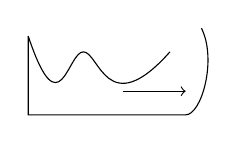
\begin{tikzpicture}
\draw (0,1) -- (0,0) -- (2,0) .. controls (2.2,0) and (2.4,.7) .. (2.2,1.1);
\draw (0,1) .. controls (.4,-.2) and (.5,.8) .. (.7,.8)
.. controls (.9,.8) and (1,-.1) .. (1.8,.8);
\draw[->] (1.2,.3) -- (2,.3);
\end{tikzpicture}}
\diagram{\begin{tikzcd}
\deleted{K} & \deleted{\mathrm{Ab}_{k*}}\arrow[l,shift left] \arrow[l,shift right,no head]
\arrow[dr,no head] &\\
&&\deleted{\unsure{\operatorname{Hom}}}
\end{tikzcd}}

\margin{\[
\rotatebox{90}{$\simeq$}\qquad\operatorname{Hom}(C_\bullet^{[n]},\lambda_\bullet^{\vee\vee})
\]
\[
\rotatebox{90}{$\simeq$}\,!\qquad(\lambda_\bullet^{\vee\vee})_{[n]}=\lambda_{[n]}^{\vee\vee}
\]
\[
\Vert\qquad k[X_{[n]}]^{\vee\vee}
\]}

R. Ainsi \unsure{on a} diagramme comm.

\margin{\[
\deleted{\unsure{\operatorname{Hom}(C_\bullet(X_*)^{\vee\vee},\Lambda^{\bullet+1}k^{\Delta^n})}}
\]
\[
\operatorname{Hom}_\bullet(\Lambda^{\bullet+1}k^{\Delta^n},C_\bullet(X_*)^{\vee\vee})
\]
\[
\rotatebox{90}{$\simeq$}\qquad\operatorname{Hom}(C^\bullet(X_*),\Lambda^{\bullet+1}k^{\Delta^n})
\]
\[
\rotatebox{90}{$\simeq$}
\]}
\figure{\begin{tikzpicture}\draw (.5,1.4) .. controls (-.4,-.2) and (0,-.8) .. (.5,-.8) -- (1.6,-.8);\end{tikzpicture}}

\diagram{\begin{tikzcd}[column sep=large,row sep=large]
X_{[n]}\arrow[d] & \operatorname{Hom}(\Delta_*^n,X_*)\arrow[dd] \arrow[l,"\simeq" description,no head]\\
k[X_{[n]}]\arrow[d,"(\text{iso si }X_n\text{ fini})"'] &\\
k[X_{[n]}]^{\vee\vee} &
\operatorname{Hom}(F\deleted{(X_*}_{\inserted{X_*}},F_{\Delta_*^n})\simeq\operatorname{Hom}(C^\bullet(X_*),C^\bullet(\Delta_*^n))
\arrow[l,"\sim"]
\end{tikzcd}}

Faisons en particulier $X_*=\Delta_*^m$, on trouve donc
\diagram{\begin{tikzcd}[column sep=large,row sep=large]
\Delta_{[n]}^m=\operatorname{Hom}(\Delta^n,\Delta^m)\arrow[d]
\arrow[r,"\simeq" description,no head] & \operatorname{Hom}(\Delta_*^n,\Delta_*^m)\arrow[d]\\
k(\Delta_{[n]}^m)\arrow[r,"\simeq" description,no head] &
\operatorname{Hom}(F_{\Delta_*^m},F_{\Delta_*^n})\simeq
\end{tikzcd}}

\mspage{340}
\scanpage{340}

\diagram{\begin{tikzcd}
k^{\operatorname{Hom}(\Delta^m,\Delta^n)} &
k^{\operatorname{Hom}(\Delta^m,\Delta^{n-1})}\arrow[l,bend right=25]
\end{tikzcd}}
\figure{\begin{tikzpicture}\draw (0,0)--(.7,.025);\end{tikzpicture}}

\diagram{\begin{tikzcd}[column sep=large]
C_{[n]}^\bullet=\deleted{\unsure{a|\alpha}}\Lambda^{\bullet+1}\Phi_{[n]}
=\Lambda^{\bullet+1}k^{\Delta^n}\arrow[r,leftrightarrow]
&\deleted{\unsure{\Phi}}\lambda^\bullet\\
C_\bullet^{[n]}\cdot\Lambda^{\bullet+1}\check\Phi_{[n]}
=\Lambda^{\bullet+1}k^{\Delta^n}\arrow[r]&\lambda_\bullet
\end{tikzcd}}
\diagram{\begin{tikzcd}
C_*^{[n]}\arrow[r]&\lambda_*
\end{tikzcd}}
\margin{$\mathbb C_{[n]}^*=\mathbb C^*(\Delta_*^n)$}
\[
\begin{aligned}
&\Vert\\
\mathbb C^*(\Delta_*^n)^\vee
&=\mathbb C_*(\Delta_*^n)\\
&=k[\Delta_*^n]
\end{aligned}
\]
\diagram{\begin{tikzcd}
C_{[n]}^\bullet\arrow[r]&K^\bullet\\
C_{[n]}^*\arrow[r,no head]&K^*
\end{tikzcd}}
\[
\begin{aligned}
\operatorname{Hom}_k(k[\Delta_*^n],\lambda_*)&=\operatorname{Hom}(\Delta_*^n,\lambda_*)\\
&=\lambda_{[n]}
\end{aligned}
\qquad C_*^*(
\]
prenons
\[
\lambda^\bullet=C^\bullet(\Delta_*^m)\simeq\Lambda^{1+i}k^{\Delta^m}
\]

\[
\operatorname{Hom}^\bullet(
\underbrace{\Lambda^{1+\bullet}k^{\Delta^m}}_{\text{avec}},
\underbrace{\Lambda^{1+\bullet}k^{\Delta^n}}_{\text{prod. ext}})
=\operatorname{Hom}^\bullet(C_{[n]}^\bullet,\lambda^\bullet)
\]
\[
\Vert
\]
\[
\operatorname{Hom}_\bullet(
\underbrace{\Lambda^{1+\bullet}k^{\Delta^n}}_{\text{avec}},
\underbrace{\Lambda^{1+\bullet}k^{\Delta^m}}_{\text{prod. int}})
\simeq\operatorname{Hom}_\bullet(C_\bullet^{[n]},\lambda_\bullet)
\]
\[
\rotatebox{90}{$\simeq$}
\]
\[
\begin{aligned}
\lambda_{[n]}&=\mathbb C_{[n]}(\Delta_*^m)
=\deleted{\mathbb C^{[n]}(\Delta_*^m)^\vee}\\
&\deleted{\simeq(k^{\operatorname{Hom}(\Delta_n,\Delta_m)})^\vee}\\
&\simeq k^{(\operatorname{Hom}(\Delta_n,\Delta_m))}
\end{aligned}
\]
\figure{\begin{tikzpicture}\draw[->](1.3,0)--(0,2.4);\end{tikzpicture}}

\diagram{\begin{tikzcd}[column sep=huge,row sep=large]
k^{\operatorname{Hom}(\Delta_n,\Delta_m)}\arrow[r]
\arrow[dr,no head,"\sim"'] &
\begin{gathered}\operatorname{Hom}_k((k^{\Delta_m},T_m),(k^{\Delta_n},T_n))\\\text{pas linéaire !}\end{gathered}\\
&\operatorname{Hom}(\Lambda^{1+\bullet}k^{\Delta_n},\Lambda^{1+\bullet}k^{\Delta_m})

\end{tikzcd}}

\mspage{341}
\scanpage{342}
\diagram{\begin{tikzcd}
 & & G\\
K\arrow[r]&F\arrow[ur]\arrow[r,shift left]\arrow[r,shift right]&F'
\end{tikzcd}}
\[
G\ (=F_{\Delta_*^n})
\]
\diagram{\begin{tikzcd}
K(M_*)\arrow[r,hook]&F(M_*)\arrow[r,shift left]\arrow[r,shift right]&F'(M_*)
\end{tikzcd}}
\[
\deleted{\unsure{C|G}(M_*)}
\]
\diagram{\begin{tikzcd}[row sep=large,column sep=large]
\Delta_*^0\arrow[d,bend left,dash]\arrow[d,bend right,dash]
 &&M_{[n]}\\
\Delta_*^1\arrow[d]&
\underset{\parallel\ F_S(K)}{K(M_*)}
\arrow[ur,"u_M",swap,"\text{$\otimes$ fonctoriel ?}"]\arrow[r]
&M_{[1]}\arrow[r,bend left,"\alpha_{M_*}^*"]
\arrow[r,bend right,"\beta_{M_*}^*",swap]&M_{[0]}\\
S
\end{tikzcd}}
\diagram{\begin{tikzcd}[column sep=large,row sep=large]
 &&&&\bullet&\\
 F_S\arrow[r]&F_{\Delta_*^1}\arrow[r,shift left]\arrow[r,shift right]
 \arrow[d,leftrightarrow]&F_{\Delta_*^0}\arrow[ddl,"i",near start]
 &k\arrow[r,Rightarrow]&\Lambda^2k^2\simeq k\arrow[r]\arrow[u]&0\\
 &{}&&k\arrow[u,"0",swap]\arrow[r,"\unsure{d_0|\mathrm{diag}}",swap]
 &k^2\arrow[u,"\Lambda T_n"]\arrow[r,shift left]\arrow[r,shift right]&k\\
 \beta T_n\wedge\beta\in&\Lambda^2\Phi_{[n]}&&&&\\
 &\alpha T_{[n]}\in k^{\Delta_n}\simeq\Phi_{[n]}\arrow[u]
 &\deleted{\operatorname{Hom}(\alpha_M^K,\beta_M^K)}
 \arrow[uur,dash]&&&
\end{tikzcd}}
\margin{$\alpha\in k$\quad $\beta\in\Psi_{[n]}$}
\[
\begin{aligned}
K(M_*)&\simeq Z^0(M_\bullet\otimes K^\bullet)\\
&\simeq\operatorname{Hom}^{\bullet}(M_\bullet^\vee,K^\bullet)\\
&\simeq\operatorname{Hom}^{*}(M_*^\vee,K^*)\\
&\simeq\operatorname{Hom}_*(K_*,M_*)
\end{aligned}
\]
\[
K_*^*\simeq\Psi_*\oplus\Lambda^2\Psi_*=
\]
\diagram{\begin{tikzcd}[column sep=large,row sep=large]
 &K(M_*)\otimes K(N_*)
 \arrow[r]\arrow[d,"\text{can.}"]
 \arrow[dl,"u_{M_*}\otimes u_{N_*}",swap]
 &M_{[1]}\otimes N_{[1]}\arrow[r,shift left]\arrow[r,shift right]
 \arrow[d,"2"]
 &M_{[0]}\otimes N_{[0]}\arrow[d,"2"]\\
 M_{[n]}\otimes N_{[n]}\arrow[d,"2"]
 &K(M_*\otimes N_*)\arrow[dl,"u_{M_*\otimes N_*}"]
 &[M\otimes N]_1\arrow[l,Leftarrow]\arrow[r,dash,shift left]\arrow[r,dash,shift right]
 &[M\otimes N]_0\\
 (M_*\otimes N_*)_{[n]}&\deleted{=M_{[n]}\otimes N}
\end{tikzcd}}
prenons $\Phi_*=C_*^0$
\diagram{\begin{tikzcd}[column sep=large,row sep=large]
K(\Phi_*)\simeq k\arrow[r]\arrow[d]
 &F_{\Delta_*^n}(\Phi_*)\simeq\Phi_{[n]}=k^{\Delta_*^n}\\
\unsure{K|P}(
\end{tikzcd}}
\[
\deleted{\operatorname{Hom}(}\qquad
\operatorname{Hom}_*(M_*,K_*
\]
\[
\deleted{K(M_*)}
\]
\[
\deleted{\operatorname{Hom}(}\qquad
\unsure{G_M|K_M}(K)=\operatorname{Hom}(M,K)
\]
\[
\operatorname{Hom}(M,K)\otimes\operatorname{Hom}(M,L)
-\operatorname{Hom}(M,K\otimes L)
\]
\[
M\longrightarrow M\otimes M
\]
\margin{\figure{\begin{tikzpicture}\draw (0,0)--(0,.35) (0,.7)--(0,1.6);\draw (.34,.1)--(.34,.35) (.34,.7)--(.34,1.65);\end{tikzpicture}}}
\mspage{343}
\scanpage{343}
\figure{\begin{tikzpicture}
\node[inner sep=12pt] (box) {\begin{minipage}{0.94\linewidth}
\diagram{\begin{tikzcd}
A\arrow[r,"u_i"]\arrow[d]&B\arrow[d,"\text{intègre}"]
&\deleted{\unsure{\sum}}&k[T]\arrow[r,dash,"u_i'"]&B\\
k&k'\arrow[l]& &T\arrow[r,|-]&b_i\\
&&&T^n\arrow[r,dash]&b_i^n
\end{tikzcd}}
\[
Y\longleftarrow X_*\qquad \sum\lambda_i b_i^n=0
\]
\[
\sum\lambda_i u_i=0\qquad
\operatorname{Ker}\underset{\inserted{\text{dists}}}{u_i}=\mathfrak p_i,\ \text{idéal premier}
\]
\[
t\in\complement\bigcup\mathfrak p_i=\bigcap\complement\mathfrak p
\]
\[
\sum\lambda_i u_i(x)^n=0\qquad\forall n
\]
\[
\deleted{u_i=u_j}\qquad u_i(x)-u_j(y)
\]
\end{minipage}};
\draw ([yshift=-.45cm]box.north west) .. controls ([yshift=.2cm]box.north west) and ([xshift=.5cm]box.north west) .. ([xshift=.9cm,yshift=.1cm]box.north west)
-- ([xshift=-.2cm,yshift=.13cm]box.north) -- ([xshift=.5cm,yshift=.04cm]box.north) -- ([xshift=-.2cm,yshift=.1cm]box.north east);
\draw ([yshift=-.45cm]box.north west) -- ([yshift=.9cm]box.south west);
\draw ([yshift=.72cm]box.south west) .. controls (box.south west) and ([xshift=.25cm,yshift=-.1cm]box.south west) .. ([xshift=.8cm,yshift=-.1cm]box.south west)
-- ([xshift=-1.2cm,yshift=-.05cm]box.south east)
.. controls ([xshift=-.5cm,yshift=.05cm]box.south east) and ([xshift=-.9cm,yshift=.6cm]box.south east) .. ([xshift=-.3cm,yshift=.7cm]box.south east)
.. controls ([yshift=.8cm]box.south east) and ([yshift=1cm]box.south east) .. ([yshift=1.3cm]box.south east)
-- ([yshift=-.1cm]box.north east);
\end{tikzpicture}}
\[
\operatorname{Hom}(\Delta_*^m,\Delta_*^n)
\xrightarrow{\sim}\operatorname{Hom}_{\mathrm{mult}}
(F_{(\Delta_*^n)},F_{(\Delta_*^m)})-
\]
\diagram{\begin{tikzcd}[column sep=large,row sep=large]
\underset{\parallel}{X_*}\arrow[r]
 &\widetilde X_*=n\mapsto\operatorname{Hom}(F_{X_*},F_{\Delta_*^n})
 \arrow[d,phantom,"\rotatebox{90}{$\simeq$}"]\\
 &\operatorname{Hom}\bigl(\varprojlim_{\Delta_*^m/X_*}F_{\Delta_*^m},F_{\Delta^n}\bigr)\\
 &\varinjlim_{\Delta_*^m/X_*}
 \underbrace{\operatorname{Hom}(F_{\Delta_*^m},F_{\Delta^n})}_{
 \simeq\ \operatorname{Hom}(\Delta_*^n,\Delta_*^m)\simeq\Delta_{[n]}^m}
 \arrow[u,"{\text{Iso?}}"{draw,ellipse}]
 \arrow[d,phantom,"\rotatebox{90}{$\simeq$}"]\\
 &X_{[n]}
\end{tikzcd}}
\margin{\deleted{$n\mapsto X_n$}}
Soient \deleted{deux}
\diagram{\begin{tikzcd}[column sep=large,row sep=large]
\overset{\substack{G\\\Vert}}{\prod F_i}\arrow[r]\arrow[d,"\pi_i",swap]&F_{\Delta_n}\\
F_i\arrow[ur,"u_i",swap]&\deleted{\sum\lambda_i u_i}
\end{tikzcd}}
\[
\prod G_i^\bullet\longrightarrow\mathbb C_{[n]}^\bullet
\]
\[
\forall M_*
\]
\[
\deleted{\prod\unsure{G_i|F_i}(M_*)\longrightarrow F(M_*)}
\]
\diagram{\begin{tikzcd}
\operatorname{Sym}G(M_*)\arrow[r,"u_i","\deleted{\operatorname{Sym}}",swap]&F(M_*)
\end{tikzcd}}
\mspage{344}
\scanpage{345}
\deleted{$F(X_*)=$}
$C^\bullet(X_*)$ avec sa structure mult. et à puiss. div.
\[
F_*(X_*)=[n\longmapsto\operatorname{Hom}(C^\bullet(X_\bullet),C(\Delta_*^n))
\]
\[
F_*(\Delta_*^{m*})=P_*^m=p_*^{m,-1}(T)
\]
\inserted{torseur sous $\check\Psi_m\otimes\Phi_*=\Phi_*^{m+1}$
(dont le gr. des sections est
$k^{m+1}\simeq\check\Psi_m$)}
\[
p_*^m:\check\Phi_m\otimes\Phi_*\longrightarrow\Phi_*
\]
\margin{(s'insérant dans}
\[
0-\check\Psi_m\otimes\Phi_*-\check\Phi_m\otimes\Phi_*-\Phi_*-0
\]
\inserted{$\operatorname{Hom}(\Phi_m,\Phi_*)$\quad $T_m\longmapsto T_*$)}
\[
\Delta_*^m\longrightarrow P_*^m\qquad y\in P_{n}^m
\]
\diagram{\begin{tikzcd}[row sep=large,column sep=large]
\deleted{\Delta_n^m=\operatorname{Hom}_{\mathrm{ens}}(\Delta^n,\Delta^m)}
\arrow[r]\arrow[dr,bend right]
&\deleted{P_n^m}\arrow[dd,bend left=60]\\
&\operatorname{Hom}(P_*^m,P_*^n)\arrow[d,bend right]\\
&\operatorname{Hom}(P^m
\end{tikzcd}}
\figure{\begin{tikzpicture}\draw (0,1.4) .. controls (1.4,1.5) and (.7,.1) .. (1.8,0) -- (2.6,0);\end{tikzpicture}}
\diagram{\begin{tikzcd}[row sep=huge]
F_*(X_*)=\operatorname{Hom}\bigl(
\varprojlim_{\Delta_*^m\in\operatorname{Ob}(\Delta)/X_*}
\deleted{\unsure{C_\bullet}}C^\bullet(\Delta_*^m),C^\bullet(\Delta_*^*)\bigr)\\
\varinjlim_{\Delta_*^m\in\operatorname{Ob}(\Delta)/X_*}
\operatorname{Hom}\bigl(\deleted{\operatorname{Hom}}(
C^\bullet(\Delta_*^m),C^\bullet(\Delta_*^*))
=\varinjlim_{\Delta_*^m\in\operatorname{Ob}(\Delta)/X_*}P_*^m
\arrow[u,"\text{isom ou équiv. d'homotopie ?}"]\\
\varinjlim_{\Delta_*^m\in\operatorname{Ob}(\Delta)}\Delta_*^m\arrow[u]
\end{tikzcd}}
\diagram{\begin{tikzcd}
\Phi_m\arrow[r]&\Phi_n\\
T_m&T_n
\end{tikzcd}}
\[
\alpha\in k,\quad\beta\in\unsure{\overline\Phi_m|\overline T_m}
\]
\[
\begin{array}{ccc}
T_0&T_1\unsure{\circ|\otimes}T_1&\cdot\\
y&T_1\circ y&y\circ T_1\\
&y\circ y&
\end{array}
\]
\diagram{\begin{tikzcd}
X_*=\operatorname{Coker}(
\Delta_*^0\arrow[r,shift left,"{\delta_0,\delta_1}"]\arrow[r,shift right]
&\Delta_*^1)
\end{tikzcd}}
\diagram{\begin{tikzcd}[row sep=large,column sep=large]
&&C^\bullet(X_*)=\operatorname{Ker}(C^\bullet(\Delta_*^1)
\arrow[r,shift left,"{C^\bullet(\delta_0),C^\bullet(\delta_1)}"]
\arrow[r,shift right]&C^\bullet(\Delta_*^0)\\
\vdots&0\arrow[d]&\vdots&\vdots\\
\Phi_m\arrow[d,"T_m\wedge",swap]
&k\arrow[l,"\alpha T_m\longleftarrow1=T_0",swap]
\arrow[r,"\mathrm{diag}"]\arrow[d,"0",swap]
&\Phi_1=k^2\arrow[d,"T_1\wedge"]
\arrow[r,bend left,"\delta_0^*=\mathrm{pr}_0"]
\arrow[r,bend right,"\delta_1^*=\mathrm{pr}_1",swap]&\Phi_0=k\\
\Lambda^2\Phi_m\arrow[d]&k\arrow[l,"T_m\wedge\beta\longleftarrow1"]
\arrow[r,"\mathrm{id}"]\arrow[d]
&\Lambda^2\Phi_1=k\arrow[d]&\vdots\\
\vdots&0&0&
\end{tikzcd}}
\margin{$(\beta\in\Phi_m)$}
\margin{$k$}
\[
F_*(X_*)=\operatorname{Hom}\bigl([0-k\xrightarrow{0}k\longrightarrow0
-\cdots],C^\bullet(\Delta_*^*)\bigr)
=\{n\longmapsto\operatorname{Hom}([-],[\Phi_n\longrightarrow\Lambda^2\Phi_n-\cdots\unsure{])\}}
\]
\inserted{(structure mult. induite par $C^\bullet(\Delta_*^1)$)}
\margin{$\alpha\in k$\quad $\beta\in T$}
\mspage{346}
\scanpage{346}
\[
d,\ \lambda=\overline T_\wedge,\ \delta,\ \mu_i=T^{(i)}\cdot,
\quad\Theta(x)=\deg(x)x
\]
\[
1,T,\overline T
\]
\[
\deleted{\Lambda\Phi\otimes\Lambda\Psi}
\]
\[
\left\{\begin{aligned}
d\lambda+\lambda d&=0&&*\\
d\delta+\delta d&=\Theta\quad\text{en degré total}\\
\delta\lambda+\lambda\delta&=\mu\\
d\mu_i-\deleted{\unsure{\mu_i d}}\mu_i d
 &=\deleted{\unsure{\lambda}}\mu_{i-1}\lambda\\
\lambda\mu_i-\mu_i\lambda&=0&&*\\
\delta\mu_i-\mu_i\delta&=0&&*
\end{aligned}\right.
\]
\[
A
\]
\[
d(T^{(n)}x)=
\underbrace{dT^{(n)}x}_{\unsure{\lambda T^{(n-1)}\overline T x|T^{(n-1)}\overline T x}}
+T^{n}dx
\]
\[
d\mu_i(x)\qquad d^\alpha\delta^\beta\lambda
\]
\[
\delta(Tx)=\deleted{\delta(T)x}+T\delta x
\]
\figure{\begin{tikzpicture}\draw (0,0)--(0,2);\end{tikzpicture}}
\[
\left\{\begin{aligned}
d\Theta-\Theta d&=0&&*\\
\delta\Theta-\Theta\delta&=0&&*\\
\Theta\lambda-\lambda\Theta&=\lambda\\
\Theta\mu_i-\mu_i\Theta&=i\mu_i
\end{aligned}\right.
\]
\figure{\begin{tikzpicture}\node[draw,ellipse,inner sep=8pt] {$\begin{gathered}
\Theta\mu_f-\mu_f\Theta=\mu_{\Theta f}\\
d\mu_f-\mu_f d=\mu_{f'}\lambda
\end{gathered}$};\end{tikzpicture}}
\[
\uline{d\lambda}\qquad\uline{\lambda\mu}\qquad\uline{\mu\delta}
\]
\figure{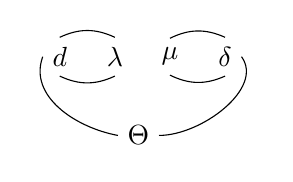
\begin{tikzpicture}
\node (d) at (0,0) {$d$};\node (l) at (.7,0) {$\lambda$};
\node (m) at (1.4,0) {$\mu$};\node (s) at (2.1,0) {$\delta$};
\node (o) at (1,-1) {$\Theta$};
\draw (d.north) to[bend left=25] (l.north);
\draw (m.north) to[bend left=25] (s.north);
\draw (d.south) to[bend right=25] (l.south);
\draw (m.south) to[bend right=25] (s.south);
\draw (d.west) .. controls (-.4,-.5) and (.2,-.9) .. (o.west);
\draw (s.east) .. controls (2.6,-.4) and (1.8,-1) .. (o.east);
\end{tikzpicture}}
\[
\frac{n(n-1)}2=\frac{5\cdot4}2=10
\qquad\frac{n(n\unsure{-|+}1)}2=\unsure{45|15}
\]
\[
d\ \delta\ \lambda\ \overset{i\ge1}{\mu_i}\ \Theta
\]
\[
\left\{\begin{aligned}
d^2=\delta^2=\lambda^2&=0\\
\mu_i\mu_j&=C_{ij}\mu_{i+j}
\end{aligned}\right.
\qquad\Theta^2\quad\text{\unsure{rien au dessus}}
\]
\[
d,\delta,\lambda
\]
\figure{\begin{tikzpicture}
\draw[rounded corners=5pt] (-.6,1.1)--(7.4,1.4)--(7.4,-1.5)--(-.6,-1.7)--cycle;
\node (d) at (0,0) {$d$};\node (l) at (.8,0) {$\lambda$};
\node (m) at (1.7,0) {$\mu_f$};\node (s) at (2.6,0) {$\delta$};
\node (o) at (1.3,-1) {$\Theta$};
\draw (0,.25)--(0,.55)--(.7,.55)--(.7,.25);
\draw (.85,.25)--(.85,.55)--(1.65,.55)--(1.65,.25);
\draw (1.8,.25)--(1.8,.55)--(2.55,.55)--(2.55,.25);
\fill (.35,.8) circle (1pt);\fill (1.2,.8) circle (1pt);
\node at (2.7,1) {$\delta(T^{(i)})=0$};
\draw (d.south) .. controls (0,-.6) and (.6,-.8) .. (o.west);
\draw (s.south) .. controls (2.6,-.5) and (1.9,-1) .. (o.east);
\fill (-.1,-.9) circle (1pt);\fill (2.6,-.9) circle (1pt);
\node[anchor=west] at (3.2,-.2) {$\left\{\begin{aligned}
&\bullet\ d^2=\delta^2=\lambda^2=0\ \bullet\\
&\bullet\ \mu_f\mu_g=\mu_{fg},\quad\unsure{\mu_{f'}=f'\mu_1}\\
&\Theta^2=-
\end{aligned}\right.$};
\end{tikzpicture}}
\[
\varphi(\lambda x)=(\deg x+i)\lambda x
\]
\[
\lambda(\varphi x)=\deg x\ \lambda x
\]
\[
\varphi\lambda-\lambda\varphi=i\lambda x
\]
\[
\overset{A}{\sum}\lambda^\epsilon\cdot
\mu_{f_{(\epsilon,}}\ ;\ \delta^{\epsilon'}\Theta^n
\]
\figure{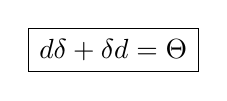
\begin{tikzpicture}\node[draw,inner sep=4pt] {$d\delta+\delta d=\Theta$};\end{tikzpicture}}
\[
\left\{\begin{aligned}
\delta\lambda+\lambda\delta&=\mu_T\\
d\mu_f-\mu_f d&=\mu_{f'}\lambda\quad\bullet\\
\Theta\lambda-\lambda\Theta&=\lambda\quad\bullet\\
\Theta\mu_f-\mu_f\Theta&=\mu_{\Theta f}\quad\bullet
\end{aligned}\right.
\]
\margin{$\delta(\overline T)=T$}
\[
\sum_{\deleted{\substack{\unsure{\alpha,\beta,\sigma,n}\\\unsure{\epsilon,\epsilon',\epsilon''}}}}
\mu_{f_{\unsure{\alpha,\beta,\sigma,n|\alpha,\beta,\sigma,}}}
\underbrace{\lambda^\alpha d^\beta\delta^\sigma\Theta^n}_{
\substack{\lambda^\epsilon d^{\epsilon'}\delta^{\epsilon''}\Theta^n\\
\epsilon,\epsilon',\epsilon''}}
\]
\margin{$\alpha,\beta,\sigma\in\mathbb F_2$\quad $n\in\mathbf N$}
\[
\deleted{\mu_f}
\]
\[
f\lambda^\alpha d^\beta\delta^\sigma\Theta^n
g\lambda^{\alpha'}d^{\beta'}\delta^{\sigma'}\Theta^{n'}
\]
\[
\lambda^\alpha\underbrace{d^\beta g}_{g d^\beta+\beta g'\lambda}
\delta^\sigma\lambda^{\alpha'}d^{\beta'}\delta^{\sigma'}
\]
Cas $p$ quelconque, $q=1$
\diagram{\begin{tikzcd}[column sep=large,row sep=large]
0\arrow[r,dash]&\Gamma^p\Phi_*\arrow[r]
&\Gamma^{p}\Phi_*\otimes\Phi_*\arrow[r,dash]
&\Gamma^{p}\Phi_*\otimes\unsure{\Phi_\alpha|\Psi_\alpha}\arrow[r]
\arrow[l,bend left=35,"?",swap]&0\\
&&&\Phi_\alpha\times\Psi_\alpha\arrow[ul]&
\end{tikzcd}}
\diagram{\begin{tikzcd}
\Gamma^{*+}\Phi_*\otimes\Lambda^{\deleted{\unsure{\epsilon}}\inserted{*}}\Psi_*\arrow[d]\\
\Gamma^{*+}\Phi_*\otimes\Lambda^*\Phi_*
\end{tikzcd}}
\[
(\varphi,\psi)\longrightarrow s(\varphi\otimes\psi)\varphi^{(p-1)}
\]
\[
\overset{\deleted{\unsure{q|p}}}{\varphi}_1^{(p_1)}-\varphi_r^{(p_r)}\qquad\sum p_i=p
\]
\diagram{\begin{tikzcd}[row sep=large]
\phantom{\varphi_1^{(p_1)}}\arrow[d]\\
\phantom{f(\varphi)}
\end{tikzcd}}
\[
\deleted{\sum\lambda_i\varphi_i}
\]
\[
\begin{aligned}
f\Bigl(\sum_i^r\lambda_i\varphi_i\Bigr)
&=s\Bigl(\sum\lambda_i\varphi_i\otimes\psi\Bigr)
\Bigl(\sum\lambda_i\varphi_i\Bigr)^{(p-1)}\\
&=\sum_{1\le i\le r}\lambda_i s(\varphi_i\otimes\psi)
\sum_{\substack{(p_1-p_r)\in\mathbf N^r\\\sum p_i=p-1}}
\lambda_1^{p_1}-\lambda_r^{p_r}\varphi_1^{(p_1)}-\varphi_r^{(p_r)}\\
&=\sum_{\substack{1\le i\le r\\(p_1-p_r)}}
\deleted{\lambda_i}\lambda_1^{p_1}\lambda_i^{p_i+1}\lambda_r^{p_r}
s(\varphi_i\otimes\psi)\varphi_1^{(p_1)}-\varphi_r^{(p_r)}
\end{aligned}
\]
\[
\varphi_1^{(q_1)}-\varphi_r^{(q_r)}\longmapsto
\sum_{\substack{\deleted{\substack{\unsure{1\le i\le r}\\1\le\alpha\le r\\q_\alpha\ge1}}\\\inserted{\alpha\in\operatorname{Supp}q}}}
s(\varphi_\alpha\otimes\psi)\varphi_1^{(q_1)}-
\varphi_\alpha^{(q_\alpha-1)}-\varphi_r^{(q_r)}
\]
\[
q_1-q_r=p
\]
\diagram{\begin{tikzcd}[row sep=large]
\Gamma^2\Phi_*\otimes\Psi_*\arrow[d,bend left=35,"?"]\\
\Gamma^2\Phi_*\otimes\Phi_*\arrow[u]\\
\Gamma^2\Phi_*\arrow[u]\\
0\arrow[u]
\end{tikzcd}}
\diagram{\begin{tikzcd}[row sep=large]
\phantom{\Gamma^q(\Phi)}\\
\Gamma^q(\Phi)\otimes\Phi\arrow[u]\arrow[d]\\
\Gamma^q(\Phi)\otimes\Psi'
\end{tikzcd}}
\figure{\begin{tikzpicture}\draw (0,0)--(2,2.8);\draw (0,-1.8)--(0,0);\end{tikzpicture}}
\[
\sum_{\alpha\in\operatorname{Supp}q}
\underbrace{(\varphi_\alpha\otimes\psi)
\varphi_1^{(q_1)}-\varphi_\alpha^{(q_\alpha-1)}-\varphi_r^{(q_r)}}_{
\displaystyle=\sum q_\alpha\psi\varphi_1^{(q_1)}-\varphi_\alpha^{(q_\alpha)}-\varphi_r^{(q_r)}}
\]
\[
\Gamma^p\Phi_*,\quad\Lambda^q\Psi_*,\quad\Lambda^r\Phi_*,
\]
\figure{\begin{tikzpicture}\node[draw,ellipse] {$\Gamma^s\Psi_*\ ?$};\end{tikzpicture}}
\[
\unsure{\gamma_p|\gamma_\rho}(\psi\varphi_1^{(q_1)}-\varphi_n^{(q_n)})
\]
\[
\Phi_*,\Psi_*
\]
\[
\left\{\begin{aligned}
\Gamma^p\Phi_*\otimes\Lambda^q\Psi_*&=\mathrm{DR}_*^{p,q}\\
\Lambda^r\Phi_*&=C_*^{r,0}
\end{aligned}\right.
\]
\mspage{347}
\scanpage{348}
$\frac12$-Algèbre différentielle $C^*$ sur Topos $\mathcal X$.

Anneau de base $k$ (commutatif)
résolution $C^*$ de $k$

\margin{ou, il suffit qu'il y ait une augmentation}

\diagram{\begin{tikzcd}
\unsure{\cdots|0} \arrow[r] & C^0 \arrow[r] & C^1 \arrow[r] & C^2 \arrow[r] & -\\
& k \arrow[u]
\end{tikzcd}}

(la section unité de $k$ correspond à une section $T$ de $C^0$)

\deleted{bilin.}

Accouplements (notés $x,y\longmapsto x\circ y$)
\[
\left\{\begin{array}{lll}
Z^i\times C^j\longrightarrow C^{i+j}&(a_{ij})\\
C^i\times Z^j\longrightarrow C^{i+j}&(b_{ij})&i,j\geq0
\end{array}\right.
\]
satisfaisant aux conditions

$1^\circ)$ $a_{ij}$ et $b_{ij}$ coïncident sur $Z^i\times Z^j$ et
y prennent valeurs dans $Z^{i+j}$. (Donc la notation
$x\circ y$ non ambiguë, elle a un sens si $dx$ \uline{ou} $dy$ est nulle.)
\deleted{donc}

$2^\circ)$ Associativité $(x\circ y)\circ z=x\circ(y\circ z)$ si deux
des trois sections locales $x,y,z$ (de $C^i,C^j,C^h$)
sont des cocycles; $1\circ x=x\circ1=x$.

\[
3^\circ)\quad\left\{\begin{array}{l}
x\circ y=y\circ x\;(-1)^{\deg y\deg x}\\
x\circ x=0\quad\text{si $x$ section locale de $Z^i$, $i$ \uline{impair}}
\end{array}\right.
\]

\deleted{si $\unsure{x^i|u^i}$ \unsure{section locale de} $C^i$, $\unsure{z^j|x^j}$ \unsure{section locale de} $Z^j$}

$4^\circ)$ Pour tout $i,j\geq1$, existe un $h_{ij}$ bilin.
\diagram{\begin{tikzcd}
\inserted{Z^i\times Z^j} & \\
\deleted{C^{i-1}\times Z^j}\arrow[r,"h_{ij}"] & C^{i+j-1}
\end{tikzcd}}
rendant le carré suivant commutatif
\figure{\begin{tikzpicture}
\node (q) {\begin{tikzcd}
B^i\times Z^j\arrow[r] & Z^{i+j}\\
C^{i-1}\times Z^j\arrow[u,"d\times\mathrm{id}"]\arrow[r,"\unsure{h_{ij}|b_{ij}}"'] & C^{i+j-1}\arrow[u,"d"']
\end{tikzcd}};
\draw[thin] ([xshift=-2pt]q.west) -- ([xshift=-2pt,yshift=-2pt]q.south west) -- ([xshift=3pt,yshift=-2pt]q.south east) -- ([xshift=3pt,yshift=8pt]q.north east);
\end{tikzpicture}}
\margin{$d(x^i\circ z^j)=dx^i\circ z^j$}

\deleted{(donc \unsure{si} $i,j\unsure{\geq|>}0$, \unsure{on a}
\[
\unsure{h_{ij}(dx^{i-1})\times z^j=d(h_{ij}(x^{i-1},z^j))}
\]
\unsure{si} $x^{i-1}$ \unsure{section locale} \illegible{3})}

\deleted{(\uline{NB} l'indétermination des $h_{ij}$ \unsure{est dans}
\[
\operatorname{Hom}_k(C^{i-1}\otimes_k Z^j,Z^{i+j-1});
\]
\unsure{celle-ci est} \illegible{2} \unsure{voulue}; on peut \unsure{exiger pour les}
\illegible{2} \unsure{donnés}, et pour des \illegible{3}.)}

\mspage{349}
\scanpage{350}
Sous ces conditions, pour tout $U\in\operatorname{Ob}\mathcal X$,
\[
\deleted{\Gamma(U}\quad
\inserted{C^*(U)=}\operatorname{Hom}(U,C^*)=\Gamma(U,C_U^*)
\]
est \deleted{un} \inserted{$k(U)$-}complexe

$\uline{k(U)}:$ \deleted{$\Gamma(U,k_U)$} anneau commutatif unitaire
$=$ \unsure{définit des structures, ce qui implique que}
\deleted{$H^*\Gamma(U,C_U^*)$}
\inserted{$H^*=H^*(C^*(U))$}
est muni d'une structure évidente d'algèbre \inserted{graduée}
(associat., unit., anticomm\unsure{utative}).
Si $C^*$ est une \uline{résolution} de $k$, on dispose pour $U$ d'un hom
\[
(1)\qquad H^*(C^*(U))\longrightarrow H^*(U,k_U).
\]

\margin{\uline{en fait}}
\unsure{Il est évident que c'est un} homomorphisme d'anneaux.
\unsure{C'est l'objet} \illegible{2} \uline{\unsure{th.}} \unsure{d'anneaux comm.}

\uline{Ex. 1} Cas où $C^*$ \unsure{est une algèbre diff. usuelle}.

\uline{Ex. 2} $\Phi$ \unsure{est un} \illegible{2}
\unsure{anneau commutatif}, \unsure{avec une} $k$-\unsure{linéarité}.
\unsure{Supposons} $k\longrightarrow\Phi$, \unsure{libre} \illegible{3}
section $T$ de $\Phi$. \unsure{Supposons que} $\unsure{i\cdot k=T}$
\unsure{on le résout par le} complexe

\diagram{\begin{tikzcd}[column sep=small]
0\arrow[r] & C^0\arrow[r]\arrow[d,equal] & C^1\arrow[r]\arrow[d,equal] & \cdots\arrow[r] & C^n\arrow[r]\arrow[d,equal] & \unsure{C^{n+1}}\arrow[r]\arrow[d,equal] & \cdots\\
0\arrow[r] & \Phi\arrow[r,"T_\wedge"'] & \Lambda^2\Phi\arrow[r,"T_\wedge"'] & \cdots\arrow[r] & \Lambda^{n+1}\Phi\arrow[r,"T_\wedge"'] & \Lambda^{n+2}\Phi\arrow[r] & \cdots
\end{tikzcd}}

est une \uline{résolution} de $k$, \unsure{on a}
\[
Z^i\simeq\Lambda^i\Psi\qquad(i\geq0)
\]

(\unsure{en supposant que} \illegible{2} \unsure{est un} \illegible{2},
\unsure{ce qui correspond au} \illegible{2} \unsure{complexe}
\diagram{\begin{tikzcd}
\unsure{0}\arrow[r] & \Lambda^{\unsure{i-1}}\Psi\arrow[r] & \Lambda^{i}\Phi\arrow[r] & \Lambda^{\unsure{i}}\Psi\arrow[r] & 0
\end{tikzcd}})

\mspage{351}
\scanpage{351}
\uline{Non-Abelian} \uline{periods} \uline{on} \uline{smooth} \uline{manifolds}

We can find from the $d$-formulae of the model a set
of integrals defining a determining set of periods for
elements of the nilpotent $\pi_1$ quotients $\{\Gamma_k\}$. There is an
analogous discussion for the higher homotopy groups.

For example suppose the model begins as $\Lambda(x_1,x_2,y)$
with $dy=x_1\wedge x_2$. Let $\omega_1,\omega_2,\eta$ denote the 1-forms in
the manifold which are the $\rho$-images of these model generators.
If $\gamma$ is a loop in $M$ based at $p$ we can form the three
ingegrals
\[
\int_\gamma\omega_1,\ \int_\gamma\omega_2,\
\int_\gamma\eta-\int_\gamma\left(\int_{\gamma_t}\omega_1\right)\omega_2
\quad{}^1
\]

The first two periods are homology invariants of
since $\omega_1$ and $\omega_2$ are closed. The third integral is a
homotopy invariant of $\gamma$ because $d\eta=\omega_1\wedge\omega_2$. If we
traverse $\gamma_1$ and then $\gamma_2$ the periods multiply like the
matrices
\[
\begin{pmatrix}1&x&z\\0&1&\uline{y}\\0&0&1\end{pmatrix}.
\]

\figure{\begin{tikzpicture}\draw (0,0)--(5,0);\end{tikzpicture}}

1\quad These iterated integrals have been considered in
a general way, by Chen. Our theory seems to guide
their efficient application to homotopy theory.

\mspage{352}
\scanpage{352}
\deleted{\[
\unsure{Z^iC^j}=\Lambda^i\Psi\times\Lambda^{j+1}\Phi
\longrightarrow\unsure{C^{i+j}}=\Lambda^{i+j+1}\Phi
\]}

On \unsure{a alors une loi} de $k$-\unsure{Algèbre graduée}
\unsure{alternée sur} $Z^i(C)=\Lambda^i\Psi$, par le
\unsure{produit extérieur}. \unsure{Question : quand et}
\unsure{comment cela se prolonge-t-il en une}
\unsure{structure de} $\unsure{\frac12|k}$-algèbre différentielle?

\diagram{\begin{tikzcd}
Z^{i+1}\otimes C^j\arrow[r,"\text{donné}"] & Z^{i+j+1}\\
C^i\times Z^j\arrow[u]\arrow[r,"\sigma_{ij}"] & C^{i+j}\arrow[u]\\
Z^i\otimes Z^j\arrow[u]\arrow[r,"\text{donné}"] & Z^{i+j}\arrow[u]\arrow[d]\\
0\arrow[u] & 0
\end{tikzcd}}
\margin{$\big]$}

L'indétermination \unsure{pour trouver} $\sigma_{ij}$ est dans
\[
\operatorname{Hom}_k(Z^{i+1}\otimes Z^j,Z^{i+j})\quad\unsure{c.a.}
\]
\[
\underbrace{\Lambda^{i+1}\Psi\otimes\Lambda^j\Psi}_
{\displaystyle\simeq\Lambda^{i+j+1}\Psi\underset{\swarrow}{\oplus}\ \substack{\text{(quelque chose}\\\text{\unsure{d'homotopie à|d'homologie à}}\ \unsure{a|0}}}
\quad\Lambda^{i+j}\Psi
\]

\mspage{353}
\scanpage{355}
$\mathcal L$
\deleted{$\underline{\operatorname{Hom}}($}
\[
\left\{\begin{aligned}
\underline{\operatorname{Hom}}_{\mathcal L}^!((\mathrm{Ss})^\circ,\mathcal B)&\simeq\underline{\operatorname{Hom}}_{\mathcal L}^!(\mathcal B_0,\mathcal B)\\
\underline{\operatorname{Hom}}_{\mathcal L}^!((\mathrm{Ss}),\mathcal A)&\simeq\underline{\operatorname{Hom}}_{\mathcal L}^!(\mathcal A_0,\mathcal A)
\end{aligned}\right.
\]
\diagram{\begin{tikzcd}
(\mathrm{Ss})^\circ\arrow[r,"F_0"] & \mathcal B_0\simeq(\mathrm{Ab}_*)^\circ\simeq(\mathrm{Ab}^{*})^\circ\\
(\mathrm{Ss})\arrow[r,no head,"G_0"] & \mathcal B
\end{tikzcd}}
\[
\left\{\begin{aligned}
\mathcal A_0&=\mathcal B_0^\circ,\quad\overset{\simeq\mathrm{Ab}_*}{\mathcal B_0}=\mathcal A_0^\circ\simeq(\mathrm{Ab}^*)^\circ\\
G_0&=(F_0)^\circ,\quad F_0=(G_0)^\circ
\end{aligned}\right.
\qquad F_0\in\mathrm{Ab}^{*}_{*}
\]
\[
\mathbb C_*\in
\]
\deleted{$\Omega_{\mathcal L}$}
\diagram{\left\{\begin{gathered}\begin{tikzcd}
\Omega_{\mathcal L}\simeq\mathcal B_0\arrow[r,hook',"\text{pl fid}"] & \mathrm{Ab}_*^\circ\simeq\mathrm{Ab}_\bullet^\circ\\
\Omega'_{\mathcal L}\simeq\mathcal A_0\arrow[r,hook',no head,"\text{pl fid}"'] & \mathrm{Ab}_*\simeq\mathrm{Ab}_\bullet
\end{tikzcd}\end{gathered}\right.}
\[
\underline{\operatorname{Hom}}(\Delta^\circ,\mathrm{Ab}_*^\circ)\simeq
\deleted{\underline{\operatorname{Hom}}(\Delta^\circ,}
(\mathrm{Ab}_*^*)^\circ
\]
\diagram{\begin{tikzcd}[column sep=small]
& & \unsure{\mathbb C^{*\alpha}|\mathbb C^{*\vee}}\arrow[dd,bend left=25]\\
& & \tikz[baseline=(z.base)]{\node(z){$\deleted{\unsure{\xi|\Delta}}$};\draw[rotate=15] (0,0) ellipse (.38 and .23);}\arrow[d]\\
\Omega\arrow[rr,bend left=25,no head]\arrow[rrr,bend left=30,no head] & F\arrow[r,no head]\arrow[rr,bend right=20,no head] & L_* & L_\bullet
\end{tikzcd}}
Cas $\mathcal A=\mathrm{Ab}$

op. contravariants de $\Omega$ dans $\mathrm{Ab}$
\[
\boxed{F(X_*)=\Omega_{*}(\mathbb C_*^{(X)})=\Omega_\bullet(\mathbb C_\bullet(X))}
\]
\[
L_\bullet\quad L_*
\]
\[
\begin{aligned}
\operatorname{Hom}_{\widehat\Delta}(X_*,L_*)&\simeq\operatorname{Hom}_{*\to}(\mathbb C_*(X_*),L_*)\simeq\operatorname{Hom}_{\unsure{\mathrm{Ens}|\ge0}}(\mathbb C_\bullet(X),L_\bullet)\\
&\simeq\underline{\operatorname{Hom}}^*(\unsure{L^*_{\ge}|L^*_*},\mathbb C^*(X))\simeq\operatorname{Hom}^\bullet(L^\bullet,\mathbb C^\bullet(X))
\end{aligned}
\]
\margin{dans une\quad $L_*$ à augm.\quad Voy. adj.}

$\mathcal A\subset\widehat{\mathcal A}$
\[
\underline{\operatorname{Hom}}(\widehat\Delta_{\mathrm{ab}}\times\mathcal A^\circ,\mathrm{Ab})\simeq\underline{\operatorname{Hom}}(\mathcal A^\circ
\]
repr. p.r. aux deux arg.
\[
\varphi\in\underline{\operatorname{Hom}}_{!}(\underset{M}{\widehat\Delta_{\mathrm{ab}}},\underset{X}{\widehat{\mathcal A}})
\subset\underline{\operatorname{Hom}}(\widehat\Delta_{\mathrm{ab}}\times\mathcal A^\circ,\mathrm{Ab})
\]
\[
\operatorname{Hom}(X,\varphi(M))=\Phi(M,X)
\]
\margin{repr. en $X$
\figure{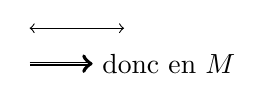
\begin{tikzpicture}
\draw[<->] (0,0)--(1.2,0);
\draw[double,->] (0,-.45)--(.8,-.45);
\node[right] at (.8,-.45) {donc en $M$};
\end{tikzpicture}}}
\deleted{$=\operatorname{Hom}(M,$}
\[
\Phi\operatorname{Hom}(\mathcal A^\circ,\underline{\operatorname{Hom}}_!,(
\]
\diagram{\begin{tikzcd}
\widehat\Delta\arrow[r,no head]&\mathrm{Ab}
\end{tikzcd}}
\diagram{\begin{tikzcd}
\underline{\operatorname{Hom}}_!(\widehat\Delta_{\mathrm{ab}},\mathcal A)\arrow[r]\arrow[dr] & \underline{\operatorname{Hom}}_!(\widehat\Delta,\mathcal A)\arrow[d,"\tikz[baseline=-.5ex]{\node[rotate=90]{$\simeq$};}"]\\
&\underline{\operatorname{Hom}}(\Delta,\mathcal A)\arrow[ul,bend left=30]
\end{tikzcd}}
\deleted{\[
X=\varinjlim_{\delta\in\Delta_{/X}}\delta
\]}
\diagram{\begin{tikzcd}[column sep=large]
\operatorname{Hom}(\varphi(X),M)=\Phi(X,M)\arrow[d,bend right=15]\arrow[dr] & : & \widehat\Delta_{\mathrm{ab}}^\circ\times\mathcal A\arrow[d]\\
\text{transf} & \text{repr. en }M & \mathrm{Ab}\\
\varinjlim\ \text{en}\\
\varprojlim\\
\text{donc repr. en }X
\end{tikzcd}}
\[
\simeq\operatorname{Hom}_{\widehat\Delta_{\mathrm{ab}}}(X,\psi(M))
\]
\diagram{\begin{tikzcd}
\widehat\Delta_{\mathrm{ab}}\arrow[r,shift left,"\varphi"] &\mathcal A\arrow[l,shift left,"\psi"]
\end{tikzcd}}
\diagram{\begin{tikzcd}
\mathcal A\arrow[r]&{}\\
\mathcal A\times\Delta\arrow[r,no head]&\mathrm{Ab}
\end{tikzcd}}
\mspage{356}
\scanpage{357}
\uline{Th Eilenberg-Zilber-Cartier}\hfill EZ 1

$X_{**}$ un \deleted{groupe}\inserted{objet} abelien bisimplical $(\qquad)$.
\deleted{\[
\unsure{N:\mathrm{Ab}(\text{bisimpl.})\longrightarrow A(}
\]}
\diagram{\begin{tikzcd}
N:A_{**}\arrow[r,"\text{eq de cat}","\sim"'] & A_{\bullet\bullet}\\
\widetilde{\phantom{X}}:A_{**}\arrow[r] & A_{\bullet\bullet}\\
\Delta:A_{**}\arrow[r] & A_*\\
\int:A_{\bullet\bullet}\arrow[r] & A_\bullet
\end{tikzcd}}
\margin{(complexe associé}
\margin{\diagram{\begin{tikzcd}
N:A_*\arrow[r] & A_\bullet\\
\widetilde{\phantom{X}}:A_*\arrow[r]&A_\bullet\\
N\arrow[r,hook]&\widetilde{(\ )}\quad\text{q ism}\\
&D(\ )\arrow[u]\quad\text{degen homot triv}
\end{tikzcd}}}

$\exists$ des \deleted{quasi-iso naturels}\inserted{morphismes} fonctoriels,
\diagram{\begin{tikzcd}
\int N\arrow[r,shift right,"\varphi"'] &N\Delta\arrow[l,shift right,"\psi"']
\end{tikzcd}}
\deleted{$X_{0,0}$}
qui coincident avec les fleches evidents en degré 0.
\figure{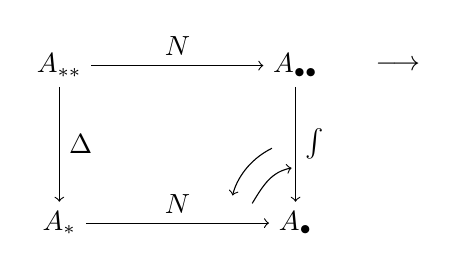
\begin{tikzpicture}
\node(a) at (0,2) {$A_{**}$};\node(b) at (3,2) {$A_{\bullet\bullet}$};
\node(c) at (0,0) {$A_*$};\node(d) at (3,0) {$A_\bullet$};
\draw[->](a)--node[above]{$N$}(b);\draw[->](a)--node[right]{$\Delta$}(c);
\draw[->](b)--node[right]{$\int$}(d);\draw[->](c)--node[above]{$N$}(d);
\node at (4.3,2) {$\deleted{\longrightarrow}$};
\draw[->](2.7,.95) .. controls (2.4,.8) and (2.25,.55) .. (2.2,.35);
\draw[->](2.45,.25) .. controls (2.6,.5) and (2.7,.65) .. (2.95,.7);
\end{tikzpicture}}
\[
\varphi\psi\sim1_{\int N}\qquad\psi\varphi\sim1_{N\Delta}
\]
\deleted{$\unsure{\varphi\psi(X_{**})}$}
\diagram{\begin{tikzcd}
\psi\varphi\int(NX_{**})\arrow[r]&\int NX_{**}\\
\varphi\psi N\Delta X_{**}\arrow[r]&N\Delta X_{**}
\end{tikzcd}}
\[
1-\psi\varphi=dk+kd\qquad1-\varphi\psi=dh+hd
\]
\diagram{\begin{tikzcd}
k:\int NX_{**}\arrow[r,shift left,"+1"]\arrow[r,shift right]&\int NX_{**}\\
h:N\Delta X_{**}\arrow[r,"+1"]&N\Delta X_{**}
\end{tikzcd}}
\figure{\begin{tikzpicture}\draw (0,0)--(4,0);\end{tikzpicture}}
\diagram{\begin{tikzcd}
\int N\arrow[r,shift left,no head,"\psi"]\arrow[d]&N\Delta\arrow[l,shift left,"\varphi"]\arrow[d,no head]\\
\int\widetilde{\phantom X}\arrow[r,shift left,"\widetilde\psi"]&\widetilde{\phantom X}\Delta\arrow[l,shift left,"\widetilde\varphi"]
\end{tikzcd}}
\deleted{$k-h'=$}
\diagram{\begin{tikzcd}
\int\widetilde{\phantom X}\arrow[r,shift right,"\widetilde\varphi"']&\widetilde{\phantom X}(\Delta)\arrow[l,shift right,"\widetilde\psi"']
\end{tikzcd}}
Si $\varphi$ et $\psi$ sont choisis, Pour un autre choix de $k',h'$
\[
k'-k=d\ell+\ell d\qquad h'-h=dm+md
\]
etc\ldots\quad$\ell$ et $m$ fonct

$\exists$ des choix traditionnels: ``application d'Alexander Whitney''
\deleted{EZ 2}
``shuffles''

\tikz[baseline=(m.base)]{\node[inner sep=0](m){cf MacLane};\draw([yshift=-2pt]m.south west)--([yshift=-2pt]m.south east);\draw([yshift=-4pt]m.south west)--([yshift=-4pt]m.south east);\draw([yshift=-6pt]m.south west)--([yshift=-6pt]m.south east);}\quad Homology
\diagram{\begin{tikzcd}
(\int\widetilde X_{**})_n=\displaystyle\bigoplus_{i+j=n}X_{(i)(j)}\arrow[r,"\text{shuffles}"]&\widetilde X_{(n,n)}\\
x_{ij}\arrow[r]&\deleted{\unsure{\sum(-1)s_\alpha s'_\beta(}}\quad x_{i+j,i+j}
\end{tikzcd}}
$(i,j)$-shuffle
\diagram{\begin{tikzcd}
(1\quad\ldots,\overset{\substack{n\\\Vert}}{i+j})\arrow[d,no head]&{}\\
s(1)\quad\ldots\quad\underbrace{s(i)}\quad\underbrace{s(i+j)}&{}
\end{tikzcd}}
\[
x_{i1}\qquad x_{i+1,i+1}
\]
\[
\sum_{0\le\alpha\le i}\unsure{(-1)_{\alpha}|(-1)^\alpha} s'_0s'_1\ldots
\overset{\deleted{\wedge}}{s_\alpha}\ldots s'_i\,x_{i1}
\]
\margin{signe$(\sigma)$}
\[
\sum_{\substack{\text{sur tout }\sigma\in\Sigma_n\\
\text{t.q. }\sigma(\alpha)<\sigma(\beta)\\
\alpha<\beta\le i\ \text{ou}\ \deleted{i<}\ i<\alpha<\beta\le n}}
\underbrace{s_{\sigma(i+1)}\ldots s_{\sigma(i+j)}}\,
\underbrace{s'_{\sigma(1)}\ldots s'_{\sigma(i)}}
\]
$\unsure{\sigma\Box|\sigma\in}$
\figure{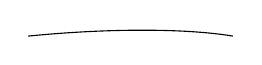
\begin{tikzpicture}\draw (0,0) .. controls (1,.1) and (2,.1) .. (2.6,0);\end{tikzpicture}}
\margin{Shuffles}
\figure{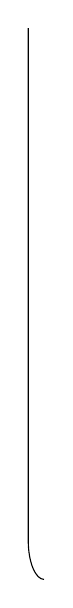
\begin{tikzpicture}
\draw (0,0)--(0,-6.5) .. controls (0,-6.8) and (.1,-7) .. (.2,-7);
\end{tikzpicture}}
\[
A\qquad\overline B(A)
\]
\figure{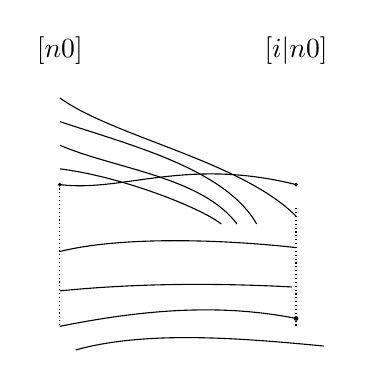
\begin{tikzpicture}[x=1cm,y=1cm]
\node at (0,2.7) {$[n\deleted{\unsure{0}}]$};
\node at (3,2.7) {$[\unsure{i|n}\deleted{\unsure{0}}]$};
\draw (0,2.1) .. controls (.7,1.6) and (2.3,1.3) .. (3,.6);
\draw (0,1.8) .. controls (.9,1.5) and (2.1,1.2) .. (2.5,.5);
\draw (0,1.5) .. controls (.7,1.2) and (1.8,1.1) .. (2.25,.5);
\draw (0,1.2) .. controls (.8,1.1) and (1.8,.7) .. (2.05,.5);
\draw (0,1) .. controls (.8,.9) and (1.6,1.35) .. (3,1);
\draw (0,.15) .. controls (.8,.35) and (2.1,.3) .. (3,.2);
\draw (0,-.35) .. controls (1,-.25) and (2,-.25) .. (2.95,-.3);
\draw[densely dotted] (0,1)--(0,-.8);
\draw[densely dotted] (3,.7)--(3,-.8);
\draw (0,-.8) .. controls (1,-.6) and (2,-.5) .. (3,-.7);
\draw (.2,-1.1) .. controls (1.1,-.85) and (2.3,-.95) .. (3.35,-1.05);
\fill (0,1) circle (.025);\fill (3,1) circle (.025);\fill (3,-.7) circle (.03);
\end{tikzpicture}}

\uuline{Alexander-Whitney}
\diagram{\begin{tikzcd}
\widehat X_{n,n}\arrow[r]&\bigoplus X_{ij}\\
x_{n,n}\arrow[r]&\displaystyle\sum_{i=0}^n(-1)^i d_0^{n-i}\widehat d^{\,i}x_{n,n}
\end{tikzcd}}
\diagram{\begin{tikzcd}[column sep=small]
\underset{f}{\underbrace{C^i(X,A)}}\otimes\underset{g}{\underbrace{C^j(X,B)}}\arrow[r,Rightarrow]&C^{i+j}(X\times X,A\otimes B)\arrow[r,bend right=15]&C^{i+j}(X,A\otimes B\\
ZX\otimes ZX&Z(X\times X)\arrow[l,Rightarrow]\arrow[r,bend right=20,no head]&{}
\end{tikzcd}}
$\widehat d$ signifie le dernier op face

$d'$ seconde op simpl.
\[
\widehat d^{\prime i}=\underbrace{d^{\prime n}d^{\prime n-1}\ldots d^{\prime n-i+1}}
\]
\[
\mathrm{E\!-\!Z\!-\!C}\Rightarrow\mathrm{E\!-\!Z}
\]
Cup-produit
\[
\left\{\begin{aligned}
h(x_1,\ldots,x_{n+1})\\
{}=\sum(-1)f(x_1\ldots x_i)g(x_{i+1},\ldots x_n)
\end{aligned}\right\}
\]
\uline{associatif}\quad(non-commutatif mais comm. à homotopie près)
\[
\Rightarrow H^*(X,R)\quad\text{est anticom.}
\]
\mspage{358}
\scanpage{358}
\diagram{\begin{tikzcd}
K(Z,i)\timesK(Z,j)\arrow[r]\arrow[d]&K(Z,i+j\\
K(Z,i)\otimesK(Z,j)\arrow[ur,"f"']&{}
\end{tikzcd}}

Il suffit de construire $Nf$
\diagram{\begin{tikzcd}[column sep=large]
N(K(Z,i)\otimesK(Z,j)\quad\cdot\arrow[dr,"\text{E.Z.}"']&&NK(Z,i+j)=Z[i+j]\\
&NK(Z,i)\otimes NK(Z,j)\arrow[ur]&{}\\
&Z[i]\overset{\Vert}{\otimes}Z[j]&{}
\end{tikzcd}}

% Deleted block: the two large diagonal strokes cross the entire parenthesized diagram.
\figure{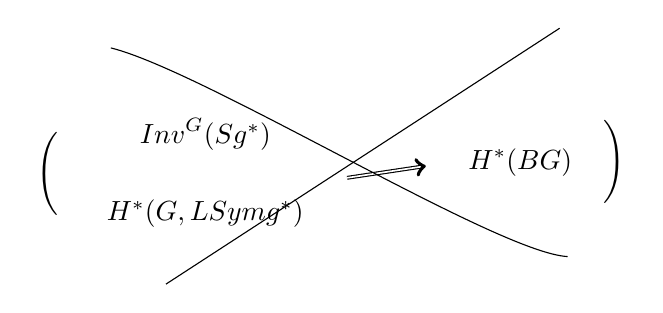
\begin{tikzpicture}
\node(a) at (0,1) {$\operatorname{Inv}^G(Sg^*)$};
\node(b) at (0,0) {$H^*(G,L\operatorname{Sym}g^*)$};
\node(c) at (4,.65) {$H^*(BG)$};
\node at (-2,.5) {$\Bigg($};\node at (5.2,.65) {$\Bigg)$};
\draw[double,->](1.8,.45)--(2.8,.6);
\draw(-1.2,2.1) .. controls (0,1.8) and (3.7,-.5) .. (4.6,-.55);
\draw(-.5,-.9)--(4.5,2.35);
\end{tikzpicture}}
\mspage{359}
